\chapter{Control System}

This chapter introduces Piranha's control system design. Unlike the simulation, where the model is 6-DoF and has a 3D environment, we based the control system design on a 3-DoF model representation, also called a navigation model. We did this because Piranha's vertical position is automatically controlled by the fluid physics. 

We also ignored the roll, pitch angles. During the field test, the collected data shows the pitch and roll angle of Piranha hardly changed. Readers can verify this fact in the simulation results.

\section{Navigation Model}

The navigation model is a 2D model rather than 3D. This is because the third position value, $z$, is not of the control system interested \cite{aastrom1976identification}. The model frame is shown in Figure \ref{fig:05nav-model}.

\begin{figure}[H]
    \centering
    \includegraphics[width=.6\textwidth]{images/05nav-model.pdf}
    \caption{Piranha navigation model and frame.}
    \label{fig:05nav-model}
\end{figure}

\subsection{Equation of Motion}

We can find the EOM of the navigation model:

\begin{equation}
    \boldsymbol{M}\dot{\boldsymbol{\nu}}+\boldsymbol{D}(\boldsymbol{\nu}, \boldsymbol{w})=\boldsymbol{\tau}
\end{equation}

Because $z,\ \phi,\ \theta$ are removed, only $p_n,\ p_e,\ \psi$ remains in the equation. The position state vector $\boldsymbol{x}_n$ and the velocity vector are defined as:

\begin{equation}
    \boldsymbol{x}_n=\left[\begin{array}{c}
        p_n  \\
        p_e  \\
        \psi
    \end{array}\right] \quad \boldsymbol{v}_n=\left[\begin{array}{c}
        u  \\
        v  \\
        r
    \end{array}\right]
\end{equation}

\subsection{Control Input}

The input vector is the same as the simulation EOM:

\begin{equation}
    \boldsymbol{\tau}=\left[\begin{array}{c}
        f_u  \\
        0 \\
        t_\tau
    \end{array}\right]=\boldsymbol{T}\left[\begin{array}{c}
        u_f  \\
        u_r 
    \end{array}\right]=\boldsymbol{T}\boldsymbol{F}_\Delta(\boldsymbol{u}_{\rm PWM})
\end{equation}

Here a new input pair $[f_f, t_r]$ is used to simplify the formulation, $f_f$ is the forward force, $t_r$ is the input torque, we can solve back from this new input vector to the original input vector simply. And with the new input representation, we have:

\begin{figure}
    \centering
    \includegraphics[width=.8\textwidth]{images/05input-loc.pdf}
    \caption{Thrusters' location with respect to the mass center.}
    \label{fig:05input-loc}
\end{figure}

\begin{equation}
    \boldsymbol{\tau}=\left[\begin{array}{cc}
        1 & 0 \\
        0 & 0\\
        0 & 1 
    \end{array}\right]\left[\begin{array}{c}
        f_f  \\
        t_r
    \end{array}\right]
\end{equation}

The reason why here a force-torque vector is the used, rather than the original PWM command vector, is that it does not break the linearity of the EOM, and on the other hand, we can search the PWM value the controller need back from the mapping function $\boldsymbol{F}_{\rm map}$. 

\begin{equation}
    \boldsymbol{u}_{\rm PWM}=\boldsymbol{F}_{\rm map}^{-1}\left(\left[\begin{array}{c}
        u_f  \\
        u_r
    \end{array}\right]\right)
\end{equation}

\subsection{Mass matrix}

The mass matrix can be written as:

\begin{equation}
    \boldsymbol{M}=\left[\begin{array}{ccc}
        m & 0 & 0 \\
        0 & m & 0 \\
        0 & 0 & I \\
    \end{array}\right]
\end{equation}

Where $m$ is the mass value of Piranha, and $I$ is the $z$ axis rotational inertia.

\subsection{Damping Matrix}

$\boldsymbol{D}(\boldsymbol{\nu})$ is the damping matrix and is much simpler than the one in simulation. We formulate it as:

\begin{equation}
    \boldsymbol{D}(\boldsymbol{\nu})=\left[\begin{aligned}
        -\frac{1}{2}A_f \rho_d u^2 & \\
        -\frac{1}{2}A_s \rho_d v^2 & \\
        -\frac{1}{2}A_I \rho_r r^2 &
    \end{aligned}\right]
\end{equation}

Where $A_f$, $A_s$, $A_I$ represent the Piranha's frontal area for $u$ $v$ and $r$ direction. $\rho_d$ is the second order drag coefficient and $\rho_r$ is the second order rotational drag coefficient.

In the end, the whole EOM can be found as:

\begin{align}
    \dot{\boldsymbol{x}} & =\left[\begin{array}{ccc}
        \cos{\psi} & -\sin{\psi} & 0  \\
        \sin{\psi} & \cos{\psi} & 0 \\
        0 & 0 & 1
    \end{array}\right]\boldsymbol{\nu} \\
    \dot{\boldsymbol{\nu}} & =\frac{1}{M}\left(\left[\begin{array}{cc}
        1 & 0 \\
        0 & 0\\
        0 & 1 
    \end{array}\right]\boldsymbol{F}_\Delta(\boldsymbol{u}_{\rm PWM})-\left[\begin{aligned}
        -\frac{1}{2}A_f \rho_d u^2 & \\
        -\frac{1}{2}A_s \rho_d v^2 & \\
        -\frac{1}{2}A_I \rho_r r^2 &
    \end{aligned}\right]\right)
\end{align}

We can see that only the $u$ and $\psi$ are controllable. The side-way speed, $v$, is constantly deteriorating because of the resistance.

\section{Extended Kalman Filter}

Piranha is equipped with multiple sensors, including two accelerometers, two gyroscopes, three magnetometers, one GPS. In such a situation, we developed an Extended Kalman Filter (EKF) for Piranha to use all the measurements to estimate the boat's position, velocity, and orientation. The full python script is attached to the Appendix \ref{app:ekf-sympy} for a better understanding of the structure of the EKF on Piranha. The mathematical formulation follows the latest EKF paper \cite{bortz1971new}, and I followed the software design criteria written on the engineering practice \cite{savage1998strapdown1, savage1998strapdown2}.

Two EKF instances run parallel on the two IMUs and output two results for the estimated states. The final result of the estimator depends on the ICM20948 EKF instance. However, another value called result credibility is calculated based on the difference between the two EKF outputs, and it decides if the EKF result is valid in the run time.

\subsection{States and Observations}

The EKF used on Piranha has 13 state variables in the state vector. These variables include:

\begin{itemize}
    \item $[q_0,q_1,q_2,q_3]$ 4 quaternions which define the orientation.
    \item $[v_n,v_e,v_d]$ NED velocity vector.
    \item $[p_n,p_e,p_d]$ NED position vector.
    \item $[{\rm mag}_N, {\rm mag}_E, {\rm mag}_D]$ NED earth fixed magnetic field components.
\end{itemize}

\begin{figure}[ht]
    \centering
    \includegraphics[width=.8\textwidth]{images/05ekf-flowchart.pdf}
    \caption{The overall EKF flowchart on Piranha.}
    \label{fig:05ekf-flowchart}
\end{figure}

\subsection{State Predict}

After getting a new set of raw data from the IMUs, the algorithm first predicts the update on the quaternions $q_0,q_1,q_2,q_3$, and the position $p_n,p_e,p_d$ in the NED frame. First the program does the following steps:

\begin{enumerate}
    \item Get raw readings from each IMU. These raw readings include the acceleration values $\Delta v_x, \Delta v_y, \Delta v_z$ from each accelerometer, and the angular speed values $\Delta a_x, \Delta a_y, \Delta a_z$ from each gyroscope.
    \item Feed the raw readings to the running integrators, save the previously estimated state vector, and check the predicted state vector's output. During this time, the values in the error matrix (sometimes called state covariance matrix $P[t+1]$) also grow.
\end{enumerate}

\subsubsection{IMU Prediction Equation}

The observation variables of the IMU includes:

\begin{itemize}
    \item $[\Delta a_x, \Delta a_y, \Delta a_z]$ Delta angular positions in the $XYZ$ frame ($xyz$ accelerations).
    \item $[\Delta v_x, \Delta v_y, \Delta v_z]$ Delta velocity in the $XYZ$ frame ($xyz$ angular velocities).
\end{itemize}

We can write the prediction equations or the discretized EOM as:

\begin{equation}
        \left[\begin{array}{c}
            v_n  \\
            v_e  \\
            v_d
        \end{array}\right]_{[t+1]}=\left[\begin{array}{c}
            v_n  \\
            v_e  \\
            v_d
        \end{array}\right]_{[t]}+\quad\left[\begin{array}{c}
            g_n  \\
            g_e  \\
            g_d
        \end{array}\right]_{[t]}{\Delta t}+Q(q_0,q_1,q_2,q_3)*\left[\begin{array}{c}
            \Delta v_x  \\
            \Delta v_y  \\
            \Delta v_z
        \end{array}\right]\Delta t_{[t]}
\end{equation}

\begin{equation}
        \left[\begin{array}{c}
            p_n  \\
            p_e  \\
            p_d
        \end{array}\right]_{[t+1]}=\left[\begin{array}{c}
            p_n  \\
            p_e  \\
            p_d
        \end{array}\right]_{[t]}+\quad\left[\begin{array}{c}
            v_n  \\
            v_e  \\
            v_d
        \end{array}\right]_{[t]}{\Delta t}
\end{equation}

\begin{equation}
        \left[\begin{array}{c}
            q_0  \\
            q_1  \\
            q_2  \\
            q_3
        \end{array}\right]_{[t+1]}=\left[\begin{array}{c}
            q_0  \\
            q_1  \\
            q_2  \\
            q_3
        \end{array}\right]_{[t]} \bigotimes\quad \left[\begin{array}{c}
            \cos{\frac{\theta}{2}}  \\
            \frac{\boldsymbol{\omega}_x}{\left\lVert\boldsymbol{\omega}\right\rVert} \sin \frac{\theta}{2}  \\
            \frac{\boldsymbol{\omega}_y}{\left\lVert\boldsymbol{\omega}\right\rVert} \sin \frac{\theta}{2}  \\
            \frac{\boldsymbol{\omega}_z}{\left\lVert\boldsymbol{\omega}\right\rVert} \sin \frac{\theta}{2}  \\
        \end{array}\right]_{[t]}\approx\quad \left[\begin{array}{c}
            q_0  \\
            q_1  \\
            q_2  \\
            q_3
        \end{array}\right]_{[t]}\bigotimes\quad \left[\begin{array}{c}
            1  \\
            0.5\Delta a_x\Delta t  \\
            0.5\Delta a_y\Delta t  \\
            0.5\Delta a_z\Delta t  \\
        \end{array}\right]_{[t]}
\end{equation}

The $[{\rm mag}_N, {\rm mag}_E, {\rm mag}_D]$ prediction equation is very simple. As we know, the earth's magnetic field barely changes locally, so the EKF predicts that these three values keep constant:

\begin{equation}
    \left[\begin{array}{c}
            \Tilde{\rm mag}_N  \\
            \Tilde{\rm mag}_E  \\
            \Tilde{\rm mag}_D
        \end{array}\right]_{[t+1]}=\left[\begin{array}{c}
            {\rm mag}_N  \\
            {\rm mag}_E  \\
            {\rm mag}_D
        \end{array}\right]_{[t]}
\end{equation}


Where $g_n,g_e,g_d$ are the gravity components in NED frame, $\mathcal{F}$ is the quaternion multiplication function.


After getting the discretized EOM, EKF calculates the Jacobian of the EOM $\boldsymbol{F}_j$ using the built-in python function \mintinline{python}{jacobian()}. Then it is used to update the covariance matrix:

\begin{equation}
    \boldsymbol{P}[t+1]=\boldsymbol{F}_j \boldsymbol{P}[t+1] {\boldsymbol{F}^\top}_j+\boldsymbol{Q}_k
\end{equation}

\subsection{Attitude Update}

Although the gyroscope provides information about the rotation angles, we need an extra step to align the starting position with the earth-fixed NED system to have the correct yaw angle. In other words, to make the North axis point to the geographical north pole. This alignment is essential for marine navigation. To do so, EKF needs a compass or magnetometer.

An extra highly sensitive magnetometer RM3100 is installed at the boat's head to generate precise yaw angle measurement.  

When EKF sees a new magnetometer measurement, the measurement is  in the body frame, so the observation function is:

\begin{equation}
    \textbf{mag}_{ob}=h(\boldsymbol{x}_{\rm EKF})=R_{\rm quat}(q_0,q_1,q_2,q_3)^\top \left[\begin{array}{c}
            \rm mag_N  \\
            \rm mag_E  \\
            \rm mag_D
        \end{array}\right]_{[t+1]}
\end{equation}

The predicted observation:

\begin{equation}
    \Tilde{\textbf{mag}}_{ob}=h(\boldsymbol{x}_{\rm EKF})=R_{\rm quat}(\Tilde{q_0},\Tilde{q_1},\Tilde{q_2},\Tilde{q_3})^\top \left[\begin{array}{c}
            \Tilde{\rm mag}_N  \\
            \Tilde{\rm mag}_E  \\
            \Tilde{\rm mag}_D
        \end{array}\right]_{[t+1]}
\end{equation}

EKF updates the attitude through:

\begin{align}
    \Delta \textbf{mag}_{ob} & =\textbf{mag}_{ob}-\Tilde{\textbf{mag}}_{ob} \\
    \textbf{H}_k &=\left.\frac{\partial h}{\partial \boldsymbol{x}}\right|_{\Tilde{x}_k} \\
    \textbf{S}_k &=\textbf{H}_k\textbf{P}_k\textbf{H}_k^\top+\textbf{R}_k \\
    \textbf{K}_k &=\textbf{P}_k\textbf{H}_k^\top\textbf{S}^{-1} \\
    \Tilde{\boldsymbol{x}}_k &=\Tilde{\boldsymbol{x}}_k+\textbf{K}_k\Delta\Tilde{\textbf{mag}}_{ob} \\
    \textbf{P}_k &=(\textbf{I}-\textbf{K}_k\textbf{H}_k)\textbf{P}_k
\end{align}

It will update both the stored magnetic field vector ${\rm mag}_N, {\rm mag}_E, {\rm mag}_D$ and the quaternions $[q0, q1, q2, q3]$.

\subsubsection{Body Magnetic Field}

In the discussion above, the calculation only considers the earth's magnetic field. However, in reality, the circuit on Piranha will inevitably create a magnetic field in the body frame. Adding the body's magnetic vector to the state vector list reduces the noise of the attitude update. However, because we installed the magnetometer on Piranha far from the electrical parts, we ignored the effect of the body's magnetic field. 


\subsection{Position Update}

EKF enters this step when there is a new position reading on the GPS sensor, a standard GPS message \textbf{\$GPSGGA} of the NMEA format contains the following information:

\begin{itemize}
    \item UTC Time.
    \item Latitude.
    \item North/South Indicator.
    \item Longitude.
    \item West/East Indicator.
\end{itemize}

The NED position measurement $p_{n{\rm GPS}},\ p_{e{\rm GPS}},\ p_{d{\rm GPS}}$ is calculated based on the latitude and longitude values first. Then it will be the observation state:

\begin{equation}
    \boldsymbol{y}_{ob}=\left[\begin{array}{c}
        p_n  \\
        p_e  \\
        p_d  \\
    \end{array}\right]
\end{equation}

So the innovation step is:

\begin{align}
    \Delta \boldsymbol{y}_{ob} & =\boldsymbol{y}_{ob}-\Tilde{\boldsymbol{y}}_{ob} \\
    \textbf{H}_k &=\left.\frac{\partial h}{\partial \boldsymbol{x}}\right|_{\Tilde{x}_k} \\
    \textbf{S}_k &=\textbf{H}_k\textbf{P}_k\textbf{H}_k^\top+\textbf{R}_k \\
    \textbf{K}_k &=\textbf{P}_k\textbf{H}_k^\top\textbf{S}^{-1} \\
    \Tilde{\boldsymbol{x}}_k &=\Tilde{\boldsymbol{x}}_k+\textbf{K}_k\Delta \boldsymbol{y}_{ob} \\
    \textbf{P}_k &=(\textbf{I}-\textbf{K}_k\textbf{H}_k)\textbf{P}_k
\end{align}

Because GPS measurements are not always available, this step will be skipped if the GPS module loses fix on the satellite and fails to obtain a new measure. In such a situation, the error matrix $P_k$ starts growing in the repeated predict steps, meaning the error accumulates in the estimated states.

\subsection{EKF Results}

Figure \ref{fig:05ekf-result-linear} and \ref{fig:05ekf-result-turn} show two EKF estimated trajectories and the raw GPS test data. We did these tests using the simulation program discussed in the previous section. We can see that, in the simulation, the EKF on Piranha can estimate the trajectory correctly even with huge GPS noise.

\begin{figure}[H]
    \centering
    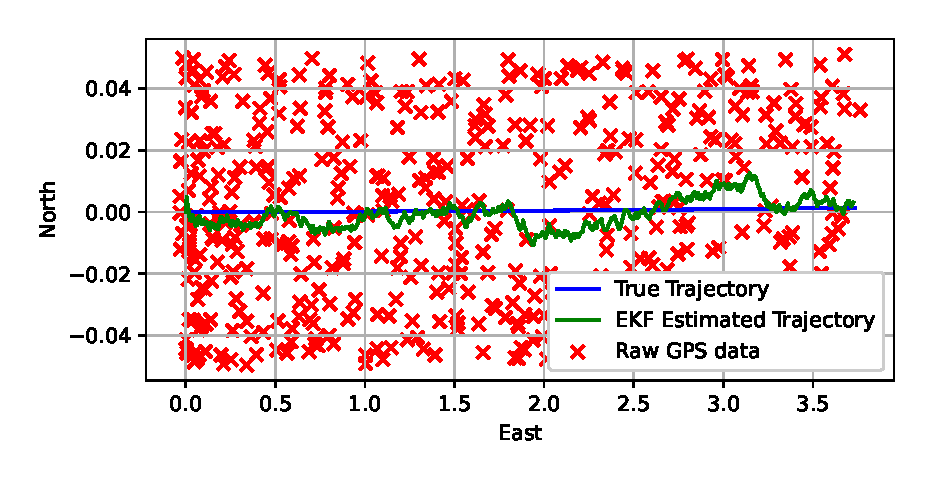
\includegraphics[width=.8\textwidth]{images/05ekf-result-linear.eps}
    \caption{EKF estimated trajectory versus raw GPS data in the linear driving simulation.}
    \label{fig:05ekf-result-linear}
\end{figure}

\begin{figure}[H]
    \centering
    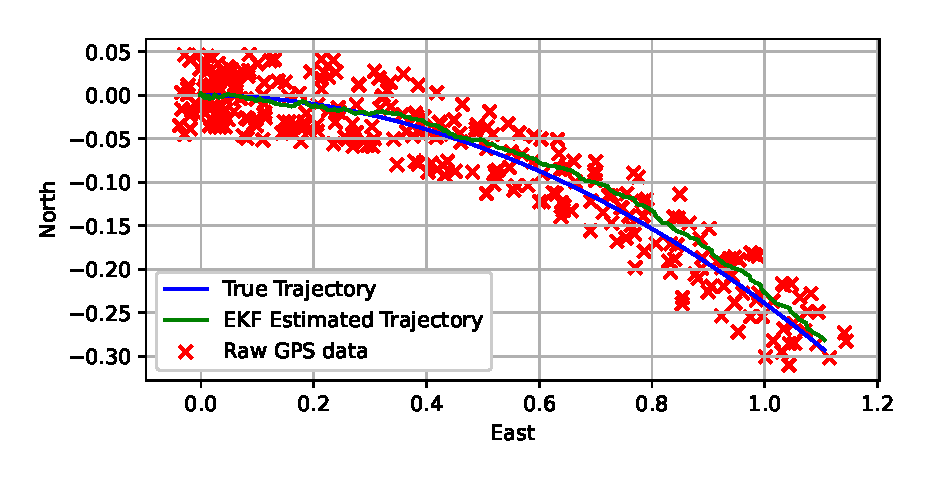
\includegraphics[width=.8\textwidth]{images/05ekf-result-turn.eps}
    \caption{EKF estimated trajectory versus raw GPS data in the steering simulation.}
    \label{fig:05ekf-result-turn}
\end{figure}

\section{PD Controller for Yaw Control}

Because there are errors in many ways, like we did not properly align the thrusters during the assembly, or one thruster is weaker than the other, the boat cannot drive in a straight line without a closed-loop controller. So a controller for yaw control driving is needed. On Piranha, A simple PD controller is implemented for this purpose. 

The key to linear driving is to keep the headings stable. We can see the structure of the PD controller in Figure \ref{fig:05pid-flowchart}.

\begin{figure}[H]
    \centering
    \includegraphics[width=.8\textwidth]{images/05pid-flowchart.pdf}
    \caption{Piranha PD heading controller flowchart.}
    \label{fig:05pid-flowchart}
\end{figure}

The PD equation is:

\begin{align}
    f_f &= k_{p1}(u-\Tilde{u}) \\
    t_r &= k_{p2}(0-\Tilde{\psi})+k_{p3}(0-\Tilde{r})+k_{d}(0- \frac{{\rm d}\Tilde{r}}{{\rm d}t})
\end{align}

After getting the $f_f$ and $t_r$, the controller solves the raw input using the reversed input mapping function:

\subsection{Test Results}

A simple test can show how the PD controller works. In the test, we reduced the left thruster's maximum power output to 80\%. Meanwhile, the right thruster is still at 100\% of the original. In real life, it is common that some ropes or plastic wastes get caught on the thruster protector and drag the left thruster down, or it is simply because the output power is different between the two thrusters due to design defections. However, we can see in Figure \ref{fig:05nopid-xyz}, \ref{fig:05nopid-ptp}, \ref{fig:05nopid-uvw}, \ref{fig:05nopid-pqr}, \ref{fig:05nopid-input} that without a PD controller, the heading $\psi$ keeps increasing, making the boat drive to the left.

\begin{figure}[ht]
    \centering
    \includegraphics[width=.8\textwidth]{images/05nopid-test-xyz.eps}
    \caption{Simulation: Without the PD controller - Positions $x, y, z$.}
    \label{fig:05nopid-xyz}
\end{figure}

\begin{figure}[ht]
    \centering
    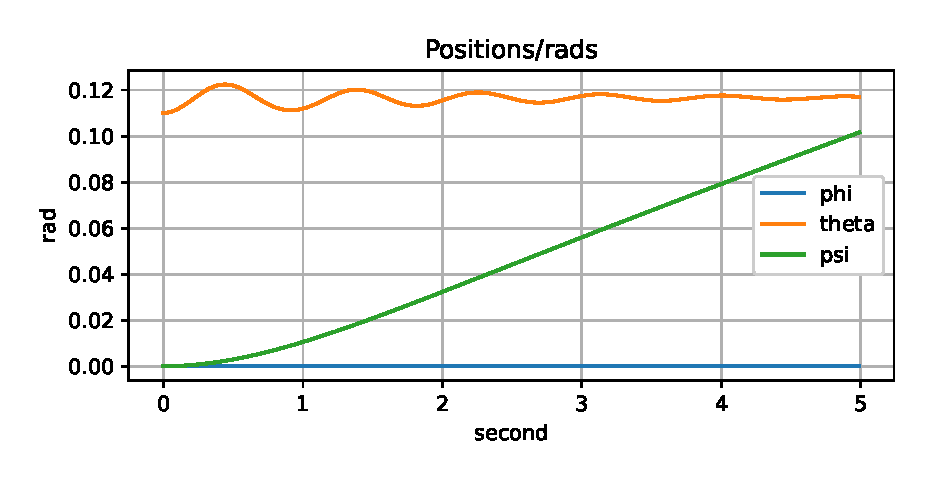
\includegraphics[width=.8\textwidth]{images/05nopid-test-ptp.eps}
    \caption{Simulation: Without the PD controller - Positions $\phi, \theta, \psi$.}
    \label{fig:05nopid-ptp}
\end{figure}

\begin{figure}[ht]
    \centering
    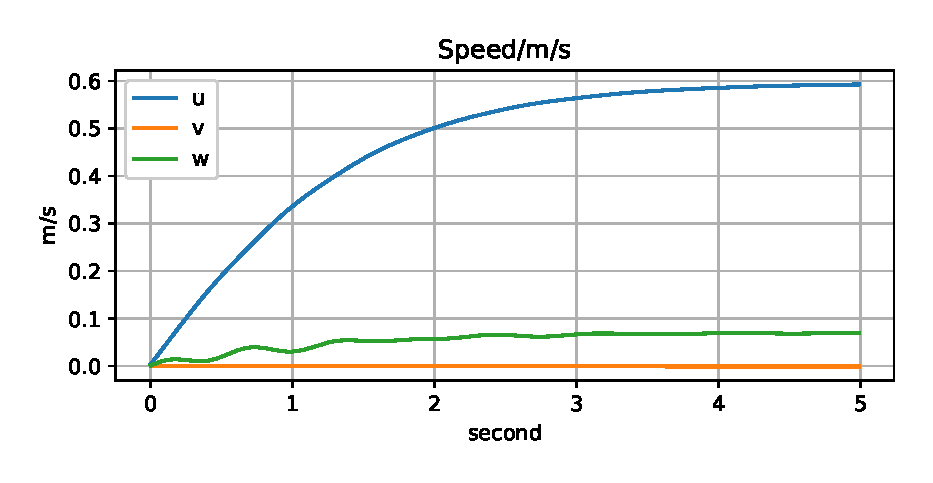
\includegraphics[width=.8\textwidth]{images/05nopid-test-uvw.eps}
    \caption{Simulation: Without the PD controller - Linear Speed $u, v, w$.}
    \label{fig:05nopid-uvw}
\end{figure}

\begin{figure}[ht]
    \centering
    \includegraphics[width=.8\textwidth]{images/05nopid-test-pqr.eps}
    \caption{Simulation: Without the PD controller - Angular Speed $p, q, r$.}
    \label{fig:05nopid-pqr}
\end{figure}

\begin{figure}[ht]
    \centering
    \includegraphics[width=.8\textwidth]{images/05nopid-test-input.eps}
    \caption{Simulation: Without the PD controller - Inputs $u_l, u_r$.}
    \label{fig:05nopid-input}
\end{figure}

With the PD controller, the input of the two thrusters are automatically calculated based on the observation to decrease the error in the heading $\psi$. The results improved by a lot, the $\psi$ stays within a small deviation range, and the drift on the $y$ direction is eliminated. The test results can be seen in Figure \ref{fig:05pid-xyz}, \ref{fig:05pid-ptp}, \ref{fig:05pid-uvw}, \ref{fig:05pid-pqr}, \ref{fig:05pid-input}.

\begin{figure}[H]
    \centering
    \includegraphics[width=.8\textwidth]{images/05pid-test-xyz.eps}
    \caption{Simulation: With the PD controller - Positions $x, y, z$.}
    \label{fig:05pid-xyz}
\end{figure}

\begin{figure}[H]
    \centering
    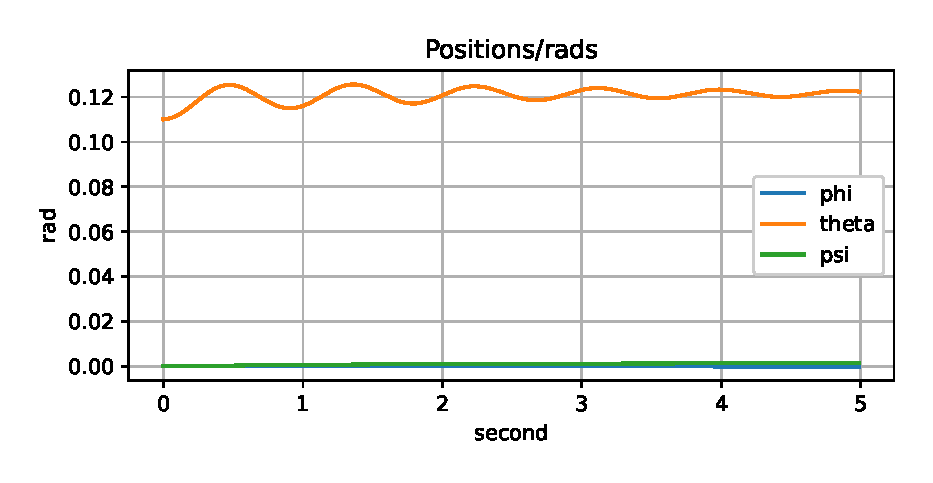
\includegraphics[width=.8\textwidth]{images/05pid-test-ptp.eps}
    \caption{Simulation: With the PD controller - Positions $\phi, \theta, \psi$.}
    \label{fig:05pid-ptp}
\end{figure}

\begin{figure}[H]
    \centering
    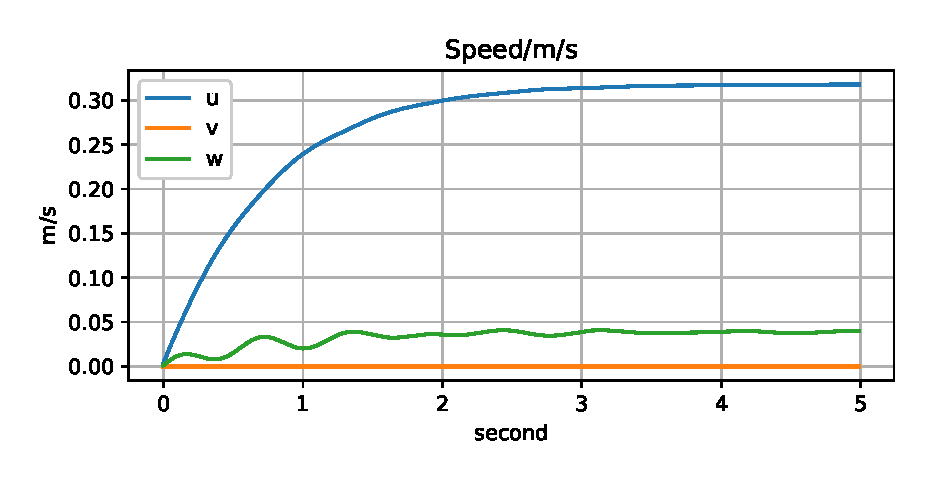
\includegraphics[width=.8\textwidth]{images/05pid-test-uvw.eps}
    \caption{Simulation: With the PD controller - Linear Speed $u, v, w$.}
    \label{fig:05pid-uvw}
\end{figure}

\begin{figure}[H]
    \centering
    \includegraphics[width=.8\textwidth]{images/05pid-test-pqr.eps}
    \caption{Simulation: With the PD controller - Angular Speed $p, q, r$.}
    \label{fig:05pid-pqr}
\end{figure}

\begin{figure}[H]
    \centering
    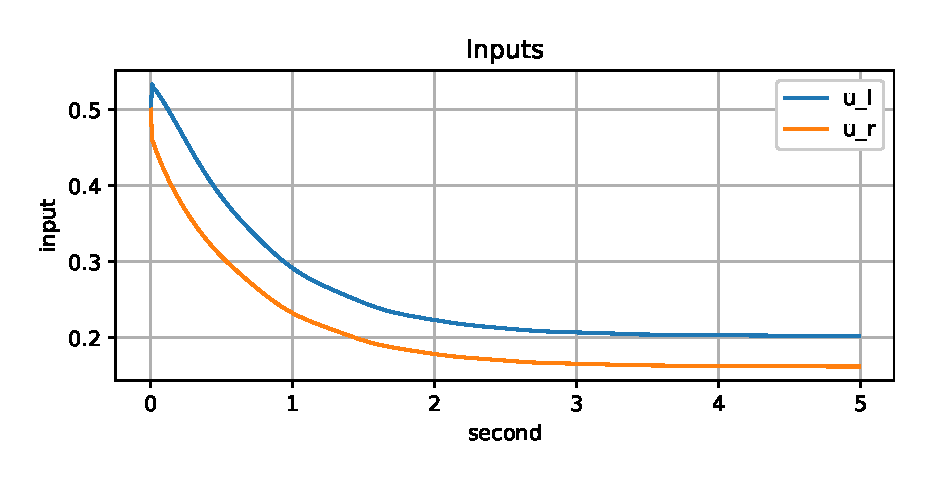
\includegraphics[width=.8\textwidth]{images/05pid-test-input.eps}
    \caption{Simulation: With the PD controller - Inputs $u_l, u_r$.}
    \label{fig:05pid-input}
\end{figure}

\section{Trajectory Tracking}

In the previous section, the PD controller can control the forward speed $u$ and the heading position $\psi$. However, the PD controller itself is not enough for Piranha to track a trajectory. This section explains the experimental trajectory tracking controller on Piranha. It was designed based on the feedback linearization theory. However, it did have the ability to correct the error one a specific direction.

In the future, I am going to test reinforcement learning and model predictive control. Previous research showed good results by using these two methods\cite{woo2018dynamic}, \cite{cuiarticle}, \cite{naeemarticle}.


\subsection{Feedback Linearization Controller}

\begin{figure}[H]
    \centering
    \includegraphics[width=.8\textwidth]{images/05fl-flowchart.pdf}
    \caption{Piranha's trajectory tracking feedback linearization controller flowchart.}
    \label{fig:05fl-flowchart}
\end{figure}

Readers can check the feedback linearization algorithm workflow in Figure \ref{fig:05fl-flowchart}. The previous section brought the EOM of the navigation model, which can be simplified as:

\begin{align}
    \dot{\boldsymbol{x}} & =\left[\begin{array}{ccc}
        \cos{\psi} & -\sin{\psi} & 0  \\
        \sin{\psi} & \cos{\psi} & 0 \\
        0 & 0 & 1
    \end{array}\right]\boldsymbol{\nu} \\
    \dot{\boldsymbol{\nu}} & =\frac{1}{M}\left(\left[\begin{array}{cc}
        1 & 0 \\
        0 & 0\\
        0 & 1 
    \end{array}\right]\boldsymbol{u}_f-\left[\begin{aligned}
        -\frac{1}{2}A_f \rho_d u^2 & \\
        -\frac{1}{2}A_s \rho_d v^2 & \\
        -\frac{1}{2}A_I \rho_d r^2 &
    \end{aligned}\right]\right)
\end{align}

To construct the feedback linearization vector, we can construct the state vector as:

\begin{equation}
    \boldsymbol{x}_l=\left[\begin{array}{c}
        p_n  \\
        p_e  \\
        \psi \\
    \end{array}\right]
\end{equation}

The observation vector is the same as the state vector with the EKF estimator brought in in the previous section.

\begin{equation}
    \boldsymbol{y}_l=\boldsymbol{x}_l
\end{equation}

Since it is a second-order system, construct a feedback vector $\boldsymbol{z}$, so that:



\begin{equation}
    \boldsymbol{z}=T(\boldsymbol{x}_l)=\left[\begin{array}{c}
        \boldsymbol{x}_l  \\
        \dot{\boldsymbol{x}}_l
    \end{array}\right]
\end{equation}

We can find the $\dot{\boldsymbol{x}}_l$ from the early EOM. Because we can directly observe the velocity vector $\boldsymbol{\nu}$ in the body frame, so its vector form is reserved. The $\ddot{\boldsymbol{x}}_l$ can be found as:

\begin{equation}
    \ddot{\boldsymbol{x}}_l=\left[\begin{array}{ccc}
        -\sin{\dot{\psi}} & -\cos{\dot{\psi}} & 0  \\
        \cos{\dot{\psi}} & -\sin{\dot{\psi}} & 0 \\
        0 & 0 & 0
    \end{array}\right]\boldsymbol{\nu}+\left[\begin{array}{ccc}
        \cos{\psi} & -\sin{\psi} & 0  \\
        \sin{\psi} & \cos{\psi} & 0 \\
        0 & 0 & 1
    \end{array}\right]\dot{\boldsymbol{\nu}}
\end{equation}

In the $\dot{\boldsymbol{\nu}}$ the input vector can be found. Define the new input of the system to be $\boldsymbol{v}$, So that the $\boldsymbol{v}$ is a linear function of $\boldsymbol{u}_f$:

\begin{equation}
    \ddot{\boldsymbol{x}}_l=f_l(\boldsymbol{u}_f)=\boldsymbol{A}_l\cdot\boldsymbol{u}_f+\boldsymbol{b}_l
\end{equation}

Which turns the given system into a linearized system with a cascade of integrators:

\begin{equation}
    \begin{split}
        \dot{\boldsymbol{z}}_1 &= z_2 \\
        \dot{\boldsymbol{z}}_2 &= \ddot{\boldsymbol{x}}_l
    \end{split}
\end{equation}

By the control law, in such a linearized system, the control vector $v$ can be found as:

\begin{equation}
    \boldsymbol{v}=-K\boldsymbol{z}
\end{equation}

After finding the control vector $\boldsymbol{v}$, the original control vector $\boldsymbol{u}_f$ can be found using the reverse mapping from $u_f\rightarrow v$.

\begin{equation}
    \boldsymbol{u}_f=A^+(\boldsymbol{v}-\boldsymbol{b})
\end{equation}

Because the matrix $A$ is not invertible, $A^+$ denotes the pseudo-inverse of the $A$ matrix. However, the primary error of the feedback linearization controller arises in this step. To explain it, we first find that:

\begin{equation}
    \left[\begin{array}{cc}
        1 & 0 \\
        0 & 0 \\
        0 & 1
    \end{array}\right]^+=\left[\begin{array}{ccc}
        1 & 0 & 0\\
        0 & 0 & 1\\
    \end{array}\right]
\end{equation}

The equation means the error in the second variable of the state $[u,\ v,\ w]$, i.e., the velocity at the $v$ direction is ignored while multiplying this matrix. We can explain this error by the fact that the system cannot control the $v$ variable. As a result, the error in the side-way direction accumulated during the trajectory, which can be seen in the next section.

\subsubsection{Circle Trajectory Result}

The first test is the circle trajectory test, the results are showed in the following Figures \ref{fig:05fl-result-circle}, \ref{fig:05fl-result-circle-xyz}, \ref{fig:05fl-result-circle-ptp},\ref{fig:05fl-result-circle-uvw},\ref{fig:05fl-result-circle-pqr}, \ref{fig:05fl-result-circle-u}. 

\begin{figure}[H]
    \centering
    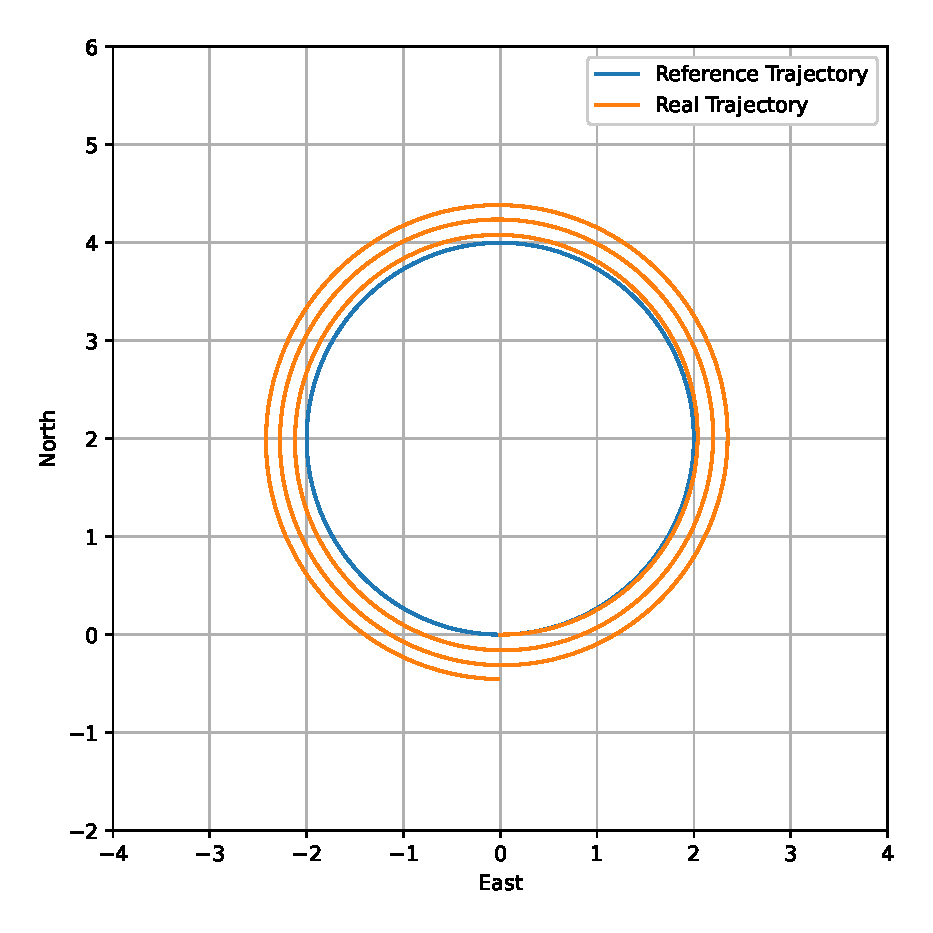
\includegraphics[width=.5\textwidth]{images/05fl-result-circle.eps}
    \caption{Feedback linearization trajectory tracking controller test result, the reference is a circle trajectory.}
    \label{fig:05fl-result-circle}
\end{figure}

\begin{figure}[H]
    \centering
    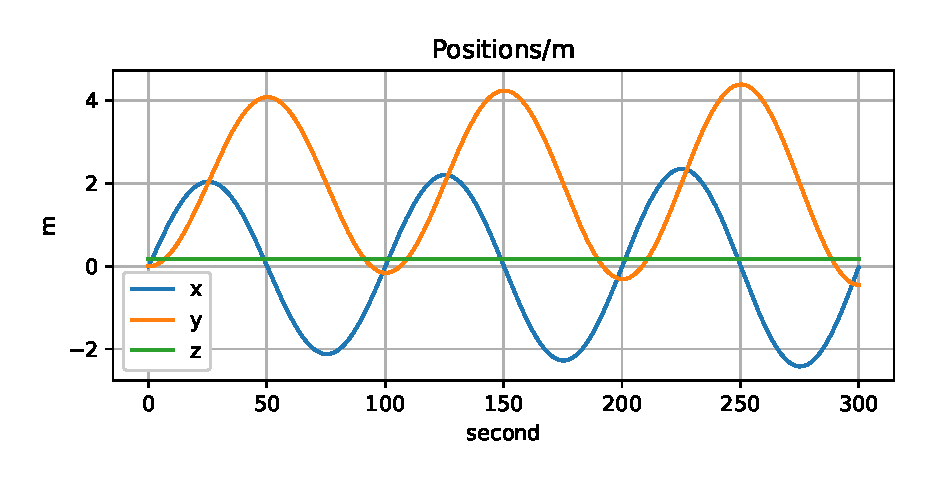
\includegraphics[width=.8\textwidth]{images/05fl-result-circle-xyz.eps}
    \caption{Feedback linearization trajectory tracking controller test result - Position $x,\ y,\ z$.}
    \label{fig:05fl-result-circle-xyz}
\end{figure}

\begin{figure}[H]
    \centering
    \includegraphics[width=.8\textwidth]{images/05fl-result-circle-ptp.eps}
    \caption{Feedback linearization trajectory tracking controller test result - Attitude $\phi,\ \theta,\ \psi$.}
    \label{fig:05fl-result-circle-ptp}
\end{figure}

\begin{figure}[H]
    \centering
    \includegraphics[width=.8\textwidth]{images/05fl-result-circle-uvw.eps}
    \caption{Feedback linearization trajectory tracking controller test result - Linear Speed $u,\ v,\ w$.}
    \label{fig:05fl-result-circle-uvw}
\end{figure}

\begin{figure}[H]
    \centering
    \includegraphics[width=.8\textwidth]{images/05fl-result-circle-pqr.eps}
    \caption{Feedback linearization trajectory tracking controller test result - Angular Speed $p,\ q,\ r$.}
    \label{fig:05fl-result-circle-pqr}
\end{figure}

\begin{figure}[H]
    \centering
    \includegraphics[width=.8\textwidth]{images/05fl-result-circle-u.eps}
    \caption{Feedback linearization trajectory tracking controller test result - Input $u_l,\ u_r$.}
    \label{fig:05fl-result-circle-u}
\end{figure}

\subsubsection{Square Trajectory Result}

The second test has a square-shaped trajectory. Compared with the circle trajectory, there are discontinuities at each vertex of the square at the reference velocity and heading. In this test, we can see that the feedback linearization controller can correct the yaw angle. However, it cannot reduce the error in the $v$ direction since the input $u_l,\ u_r$ does not control $v$ directly.

\begin{figure}[H]
    \centering
    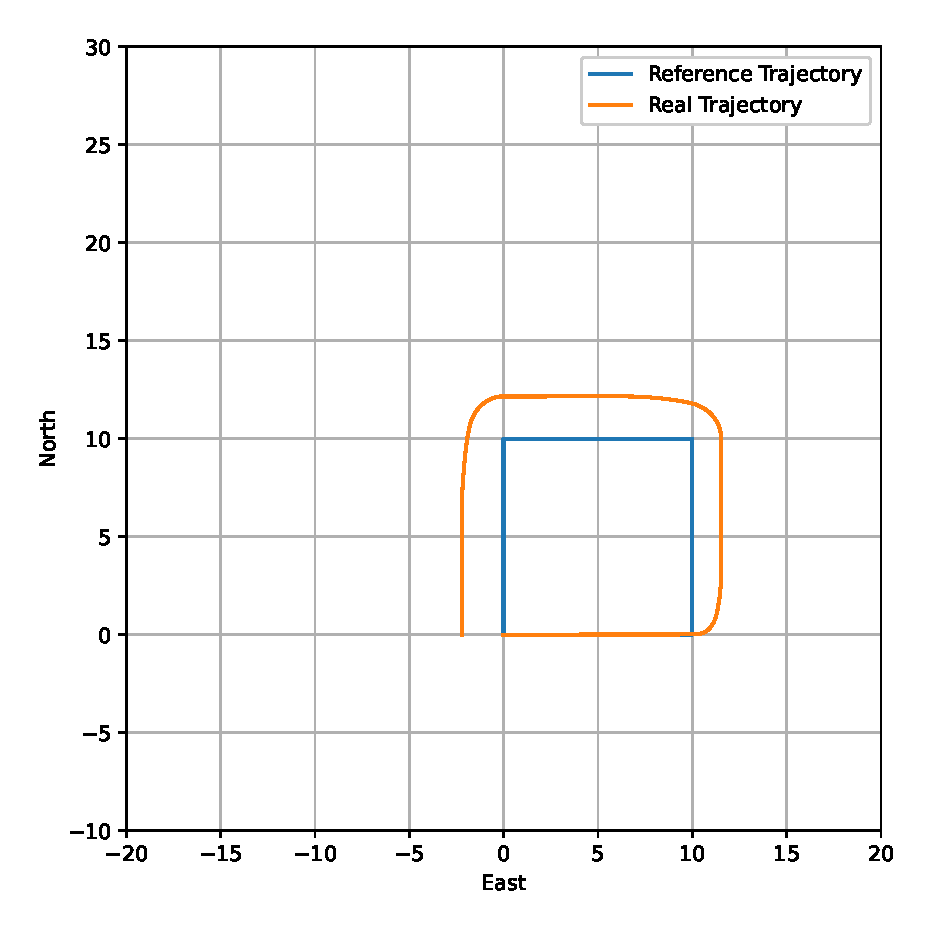
\includegraphics[width=.5\textwidth]{images/05fl-result-square.eps}
    \caption{Feedback linearization trajectory tracking controller test result, the reference is a square trajectory.}
    \label{fig:05fl-result-square}
\end{figure}

\begin{figure}[H]
    \centering
    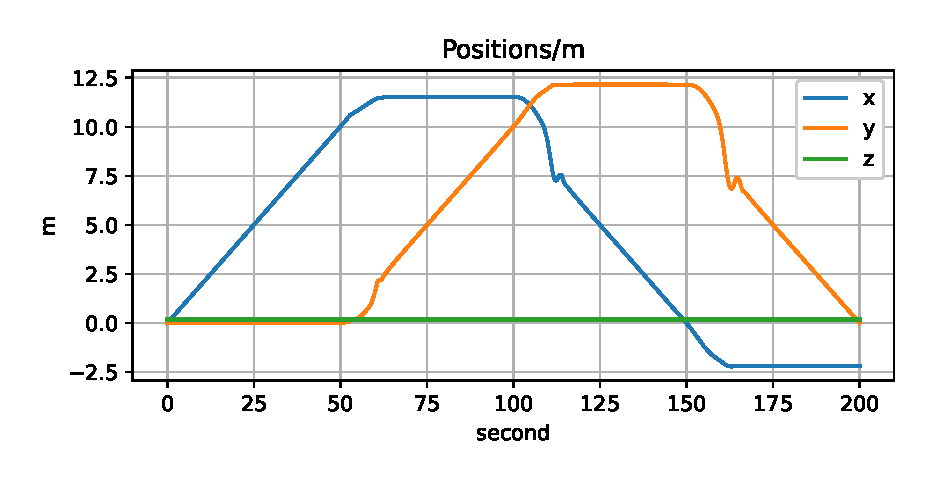
\includegraphics[width=.8\textwidth]{images/05fl-result-square-xyz.eps}
    \caption{Feedback linearization trajectory tracking controller test result - Position $x,\ y,\ z$.}
    \label{fig:05fl-result-square-xyz}
\end{figure}

\begin{figure}[H]
    \centering
    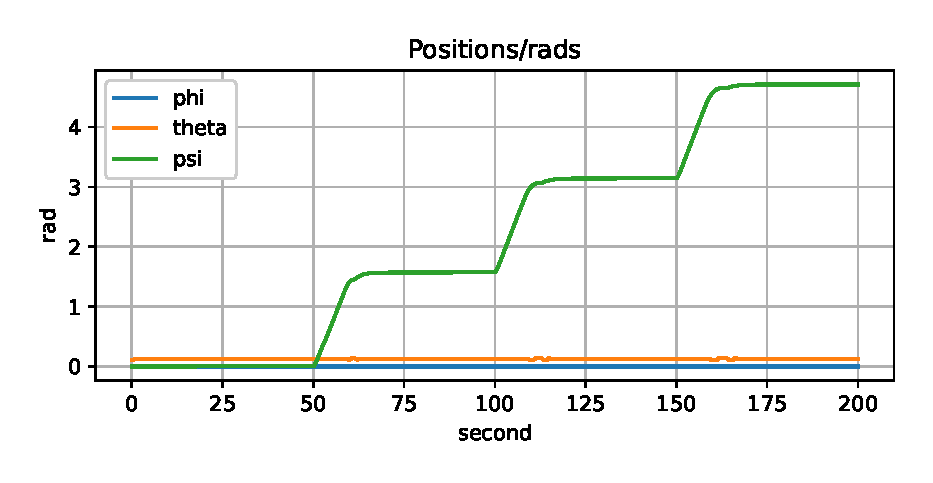
\includegraphics[width=.8\textwidth]{images/05fl-result-square-ptp.eps}
    \caption{Feedback linearization trajectory tracking controller test result - Attitude $\phi,\ \theta,\ \psi$.}
    \label{fig:05fl-result-square-ptp}
\end{figure}

\begin{figure}[H]
    \centering
    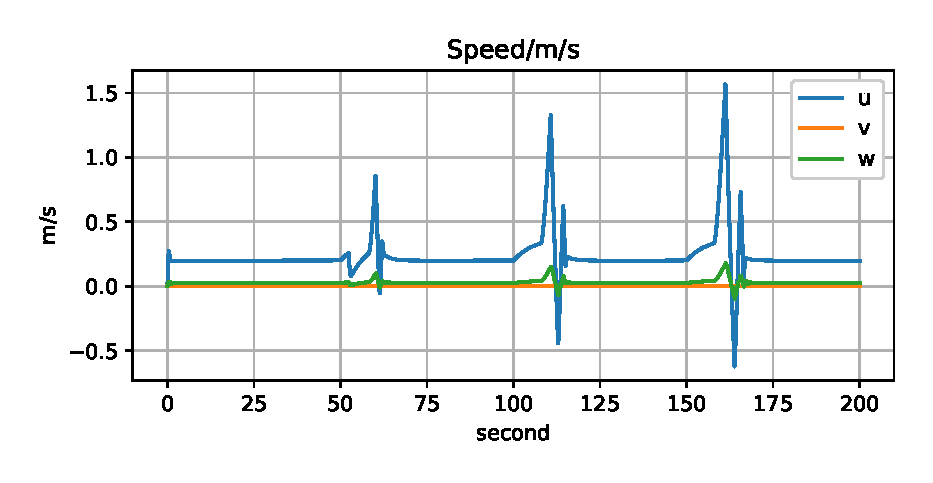
\includegraphics[width=.8\textwidth]{images/05fl-result-square-uvw.eps}
    \caption{Feedback linearization trajectory tracking controller test result - Linear Speed $u,\ v,\ w$.}
    \label{fig:05fl-result-square-uvw}
\end{figure}

\begin{figure}[H]
    \centering
    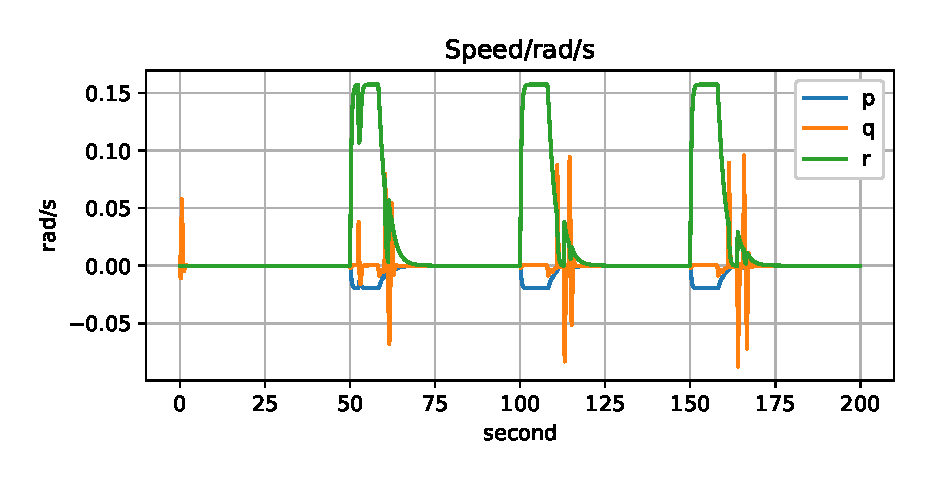
\includegraphics[width=.8\textwidth]{images/05fl-result-square-pqr.eps}
    \caption{Feedback linearization trajectory tracking controller test result - Angular Speed $p,\ q,\ r$.}
    \label{fig:05fl-result-square-pqr}
\end{figure}

\begin{figure}[H]
    \centering
    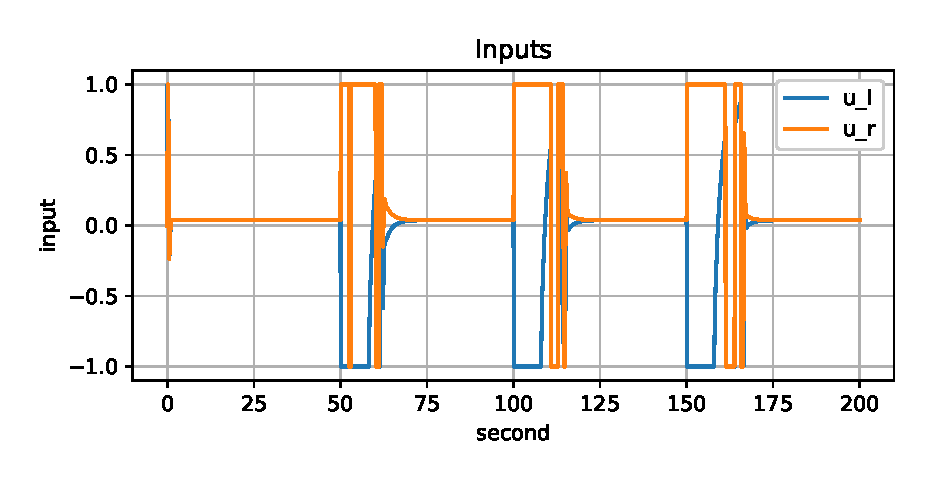
\includegraphics[width=.8\textwidth]{images/05fl-result-square-u.eps}
    \caption{Feedback linearization trajectory tracking controller test result - Input $u_l,\ u_r$.}
    \label{fig:05fl-result-square-u}
\end{figure}

We can see that the feedback linearization controller can navigate Piranha to drive towards the expected trajectory. However, because it only considers the error at present, it cannot eliminate the error at the $v$ direction, which requires the controller to have the ability to plan. 